% @author nicolas.guelfi 
% @date Tue Nov 05 17:26:22 CET 2013
%-------------------------------------------------------------------------------
% Copyright (c) 2013 University of Luxembourg.
% All rights reserved. This program and the accompanying materials
% are made available under the terms of the Eclipse Public License v1.0
% which accompanies this distribution, and is available at
% http://www.eclipse.org/legal/epl-v10.html
% 
% Contributors:
%     Alfredo Capozucca - initial API and implementation
%     Benoit Ries - minor updates
%     Nicolas Guelfi - most content from messirbook
%-------------------------------------------------------------------------------
%%%%%%%%%%%%%%%%%%%%%%%%%%%%%%%%%%%%%%%%%%%%%%%%%%
\PassOptionsToPackage{usenames,svgnames,table}{xcolor}
\documentclass[graybox,envcountchap,sectrefs,11pt]{book} 
%%%%%%%%%%%%%%%%%%%%%%%%%%%%%%%%%%%%%%%%%%%%%%%%%%
%%% DO NOT CHANGE THE ORDER 
\usepackage{./../lu.uni.lassy.excalibur.standard.report.libraries/styles/style-messir-common}
\usepackage{./../lu.uni.lassy.excalibur.standard.report.libraries/styles/style-messir-report-post}
 
%--------------------------------------------
% DOCUMENT BEGIN
%---------------------------------------- ---
\begin{document} 

\newgeometry{textwidth=17cm,textheight=23.7cm} 


\newcommand{\msrReportType}{\emph{Report type: Simulation}} 


\input{./../lu.uni.lassy.excalibur.standard.report.libraries/defs/msr-def.tex}
%  General Messir Glossary
\newglossaryentry{real number}
{name={real},
description={name of the set of real numbers},
plural={reals},
symbol={\ensuremath{\mathbb{R}}}
}

\newglossaryentry{systop}
{name={\msrglsstyle{system operation}},
description={a functionality of the system that can be triggered by a message sent by an actor belonging to the environment.},
plural={system operations},
symbol={\msrglsstyle{system operation}}
}

\newglossaryentry{protmod}
{name={\msrglsstyle{Protocol Model}},
description={},
plural={protocol models},
symbol={\msrglsstyle{protocol model}}
}

\newglossaryentry{societics}
{name={\msrglsstyle{Societics}},
description={Represents the fields of hardware/software
systems used for the society extension.},
symbol={\msrglsstyle{societics}}
}

\newglossaryentry{direct actor}
{name={\msrglsstyle{direct actor}},
description={an actor that interacts directly with the system. It thus belongs to the environment.},
plural={direct actors},
symbol={\msrglsstyle{direct actor}}
}

\newglossaryentry{indirect actor}
{name={\msrglsstyle{indirect actor}},
description={an actor that interacts indirectly with the system through a direct actor. It thus belongs the domain but not to the environment.},
plural={\msrglsstyle{indirect actors}},
symbol={\msrglsstyle{indirect actor}}
}

\newglossaryentry{abstract actor}
{name={\msrglsstyle{abstract actor}},
description={an actor that is not },
plural={\msrglsstyle{abstract actors}},
symbol={\msrglsstyle{abstract actor}}
}

\newglossaryentry{socext}
{name={\msrglsstyle{Society extension}},
description={The society obtained by grouping people using natural means
extended with artificial means.},
symbol={\msrglsstyle{societics}} }

\newglossaryentry{usecase}
{name={\msrglsstyle{Use case}},
description={A use case describes a sequence of actions that provide something
of measurable value to an actor. and is drawn as a horizontal ellipse.},
symbol={\msrglsstyle{Use case}} 
plural={\msrglsstyle{Use cases}} }

\newglossaryentry{actor}
{name={\msrglsstyle{actor}},
description={An actor is a person, organization, or external system that plays a role in one or more interactions with the system},
plural={actors},
symbol={\msrglsstyle{actor}}
}

\newglossaryentry{socialware}
{name={\msrglsstyle{Societics}},
description={Represents the fields of hardware/software
systems used for the society extension.},
symbol={\msrglsstyle{Societics}}
}

\newglossaryentry{system operation}
{name={system operation},
description={a functionality of the system that can be triggered by a message sent by an actor belonging to the environment.},
plural={system operation},
symbol={\msrglsstyle{system operation}}
}




% \newglossaryentry{}
% {name={\msrglsstyle{}},
% description={},
% symbol={\msrglsstyle{actor}} }

\newcommand{\msrprojectname}{\emph{lu.uni.lassy.excalibur.standard.specification.libraries}~} 
\newcommand{\excaliburstandardlibraries}{\emph{\msrexcalibur Standard Libraries}~} 

\newcommand{\msrReportAuthors}{} 

\newcommand{\msrReportAffiliation}{
\begin{tabular}{l}
        Laboratory for Advanced Software Systems\\
        University of Luxembourg\\
\end{tabular}
} 

\newcommand{\msrReportTitle}{
\begin{tabular}{|>{\centering\arraybackslash\hspace{0pt}}p{12cm}|}
\hline
        \textbf{\msrexcalibur Standard Libraries}\\
        \textbf{Documentation}\\
        \textbf{- v 1.4  - }\\
        \vspace{.5cm}
        {\large(\msrReportType) }\\
\hline
\end{tabular}
}


%TITLE
%******************************************
\title{
\freeblock{10}{2}{5}{
\scalebox{1.3}{\parbox{\linewidth}{
\msrReportTitle}
}}
\vspace{2cm}
\freeblock{5}{10}{-.8}{
\begin{figure}
  \centering
  
\includegraphics[width=6cm,natwidth=5847,natheight=7135]{./../lu.uni.lassy.excalibur.standard.report.libraries/logos/Messir-no-OS-focused.eps} 
\end{figure}
}
\freeblock{5}{12.5}{-.8}{
\begin{figure}
  \centering
  
\includegraphics[width=5.63cm,natwidth=5256,natheight=6852]{./../lu.uni.lassy.excalibur.standard.report.libraries/logos/Excalibur-no-OS-focused.eps}
\end{figure}
\freeblock{5}{1}{1.5}{
\scalebox{.9}{\parbox{\linewidth}{
\msrReportAffiliation
\msrReportAuthors
}}}
\freeblock{10}{5}{10}{
\scalebox{.9}{\parbox{\linewidth}{
\today~-~\currenttime
}}}
}
}
%******************************************
\author{}

\date{}
%****************************************************


\maketitle
\newpage

%TOC
\setcounter{tocdepth}{2}
\addtocounter{secnumdepth}{2}
\tableofcontents
\newpage

%TOF 
\listoffigures
\newpage

%TOL
\lstlistoflistings
\newpage

%DOCUMENT STRUCTURE
% Last Modification:
% @author AUTHOR_NAME
% @date TODAY_DATE

\chapter{Introduction}
\label{chap:introduction}
\newpage

% Last Modification:
% @author AUTHOR_NAME
% @date TODAY_DATE

\chapter{General Description}
\label{chap:general_description}

\section{Use Cases Model}
\label{sec:lu.uni.lassy.excalibur.standard.specification.libraries-gendescr-usecasemodel}

This section contains the use cases elicited during the requirements elicitation phase.
The use cases are textually described as suggested by the \msrmessir method and inspired by the standard Cokburn template~\cite{armour01usecase}.


%% ***************************************************************
%% Use Cases
\subsection{Use Cases}


There are no elements in this category in the system analysed.




%% ***************************************************************
%% Use Case Instances
\pagebreak
\subsection{Use Case Instance(s)}

There are no elements in this category in the system analysed.



\chapter{Environment Model}
\label{chap:lu.uni.lassy.excalibur.standard.specification.libraries-EM}


\section{Environment model view(s)}		
There are no view(s) for the \msrmessir environment model.



\section{Actors and Interfaces Descriptions}
\label{sec:lu.uni.lassy.excalibur.standard.specification.libraries-EM-Actors-Descriptions}

There are no elements in this category in the system analysed.




\chapter{Concept Model}
\label{chap:lu.uni.lassy.excalibur.examples.icrash-CM}


\section{PrimaryTypes-Classes}
\subsection{Local view 01}
\label{sec:lu.uni.lassy.excalibur.examples.icrash-CM-view-local-PrimaryTypes-Classes-01}
Figure \ref{fig:lu.uni.lassy.excalibur.examples.icrash-CM-view-local-PrimaryTypes-Classes-01} 
shows the local view on all the primary types class types.



\begin{figure}[htbp] 
\label{fig:lu.uni.lassy.excalibur.examples.icrash-CM}
\begin{center}
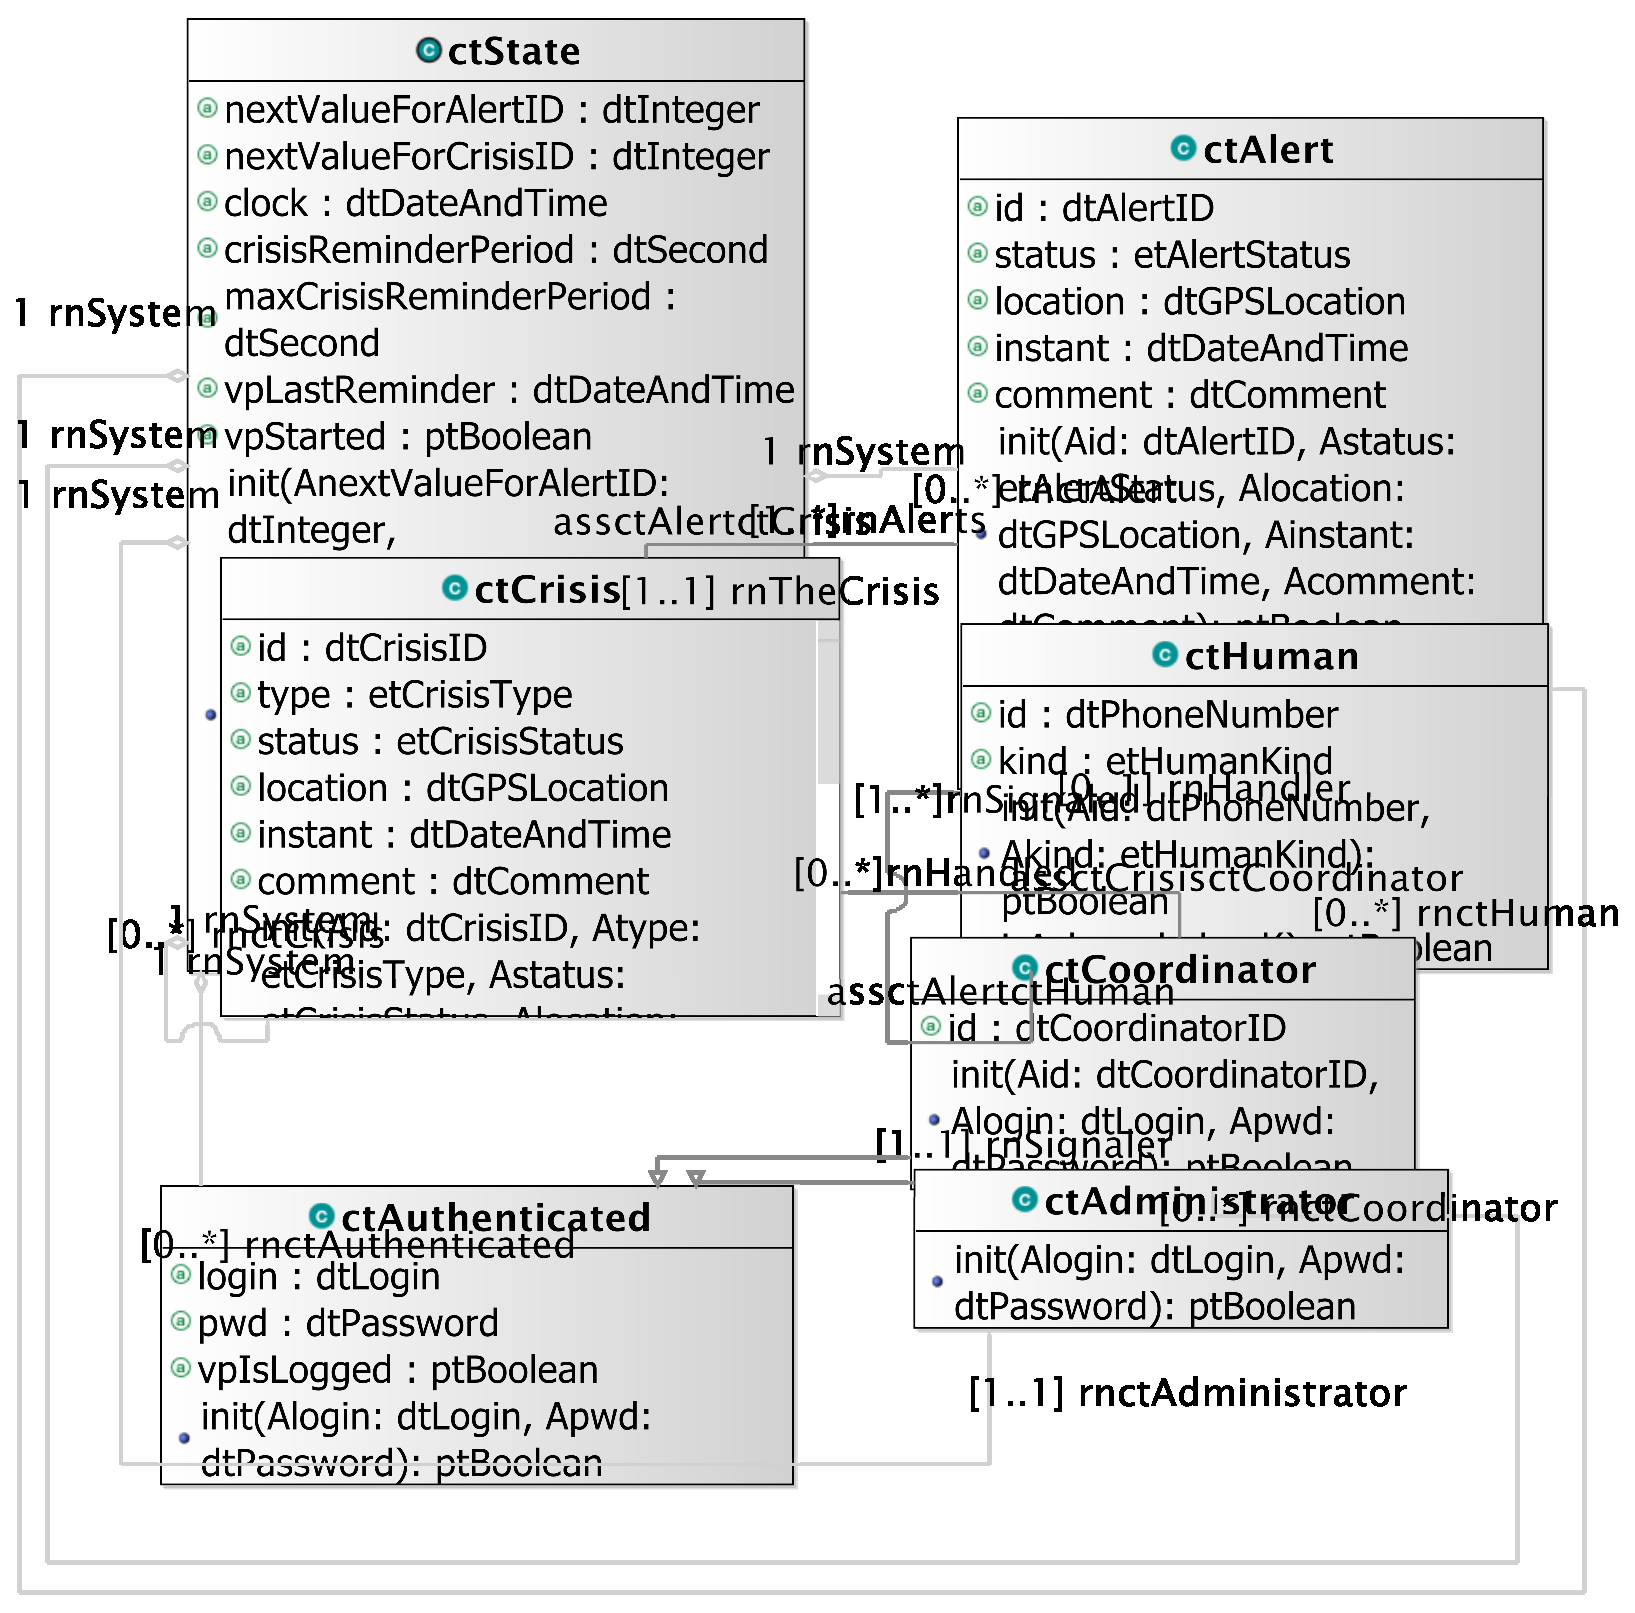
\includegraphics[
angle=0
,width=1.0\textwidth
]{./images-report-gen/concept-model/local/PrimaryTypes-Classes/01/cm-pt-ct-lv-01.eps}
\end{center}
\caption[Concept Model - PrimaryTypes-Classes local view 01 - Local view of all the primary types ]{Concept Model - PrimaryTypes-Classes local view 01. Local view of all the primary types class types
.}
\label{fig:lu.uni.lassy.excalibur.examples.icrash-CM-view-local-PrimaryTypes-Classes-01}
\end{figure}
\vspace{0.5cm} 

\subsection{Local view 02}
\label{sec:lu.uni.lassy.excalibur.examples.icrash-CM-view-local-PrimaryTypes-Classes-02}
Figure \ref{fig:lu.uni.lassy.excalibur.examples.icrash-CM-view-local-PrimaryTypes-Classes-02} shows the local view of the ctState primary type class type.



\begin{figure}[htbp] 
\label{fig:lu.uni.lassy.excalibur.examples.icrash-CM}
\begin{center}
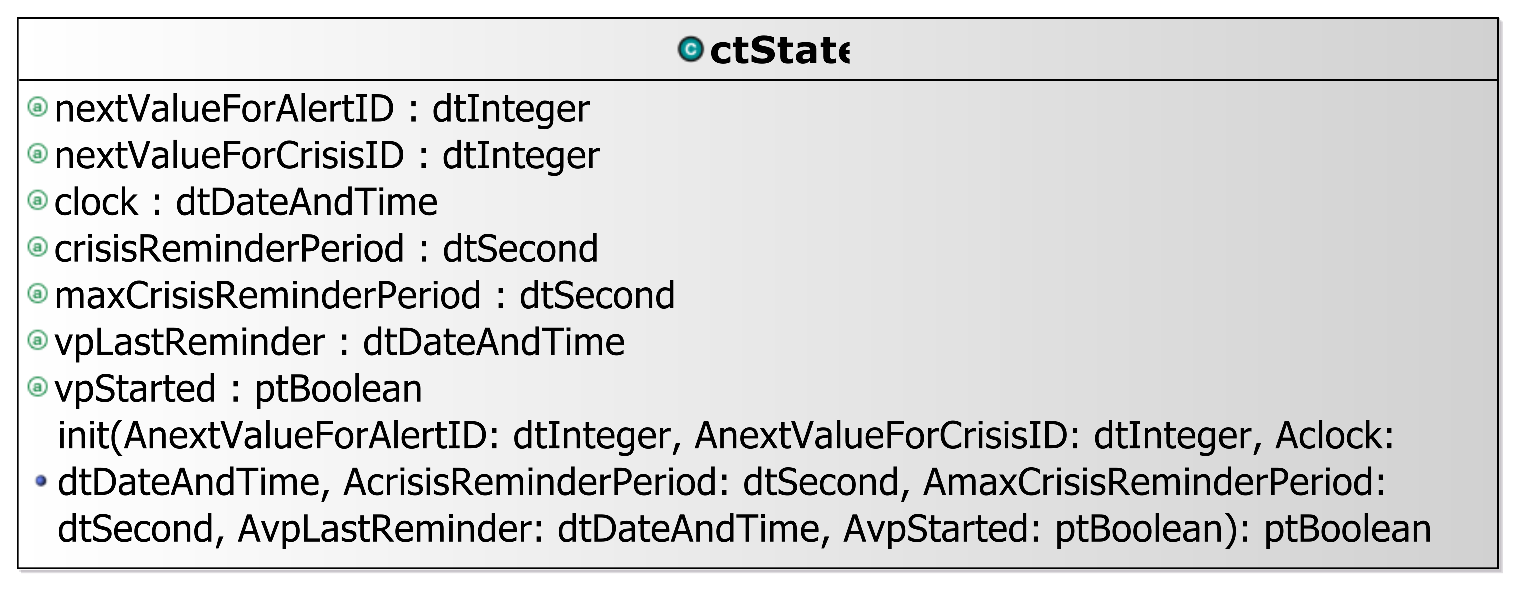
\includegraphics[
angle=0
,scale=0.80
]{./images-report-gen/concept-model/local/PrimaryTypes-Classes/02/cm-pt-ct-lv-02-parta-ctState.eps}
\end{center}
\caption[Concept Model - PrimaryTypes-Classes local view 02 - local view of the ctState primary ty]{Concept Model - PrimaryTypes-Classes local view 02. local view of the ctState primary type.}
\label{fig:lu.uni.lassy.excalibur.examples.icrash-CM-view-local-PrimaryTypes-Classes-02}
\end{figure}
\vspace{0.5cm} 

\subsection{Local view 03}
\label{sec:lu.uni.lassy.excalibur.examples.icrash-CM-view-local-PrimaryTypes-Classes-03}
Figure \ref{fig:lu.uni.lassy.excalibur.examples.icrash-CM-view-local-PrimaryTypes-Classes-03} shows the local view of the ctAlert primary type class type.



\begin{figure}[htbp] 
\label{fig:lu.uni.lassy.excalibur.examples.icrash-CM}
\begin{center}
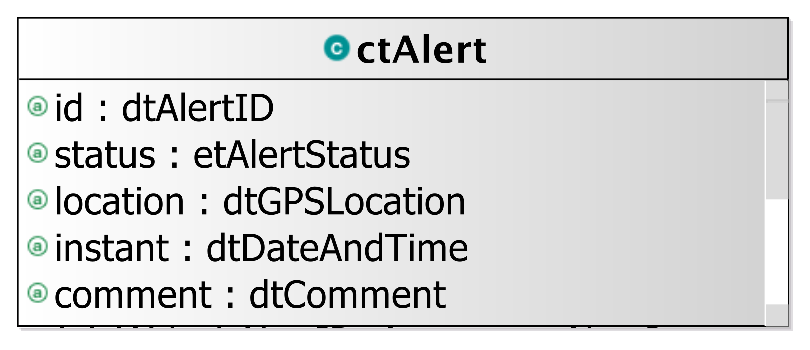
\includegraphics[
angle=0
,scale=0.80
]{./images-report-gen/concept-model/local/PrimaryTypes-Classes/03/cm-pt-ct-lv-03-partb-ctAlert.eps}
\end{center}
\caption[Concept Model - PrimaryTypes-Classes local view 03 - local view of the ctAlert primary ty]{Concept Model - PrimaryTypes-Classes local view 03. local view of the ctAlert primary type.}
\label{fig:lu.uni.lassy.excalibur.examples.icrash-CM-view-local-PrimaryTypes-Classes-03}
\end{figure}
\vspace{0.5cm} 

\subsection{Local view 04}
\label{sec:lu.uni.lassy.excalibur.examples.icrash-CM-view-local-PrimaryTypes-Classes-04}
Figure \ref{fig:lu.uni.lassy.excalibur.examples.icrash-CM-view-local-PrimaryTypes-Classes-04} shows the local view of the ctCrisis primary type class type.



\begin{figure}[htbp] 
\label{fig:lu.uni.lassy.excalibur.examples.icrash-CM}
\begin{center}
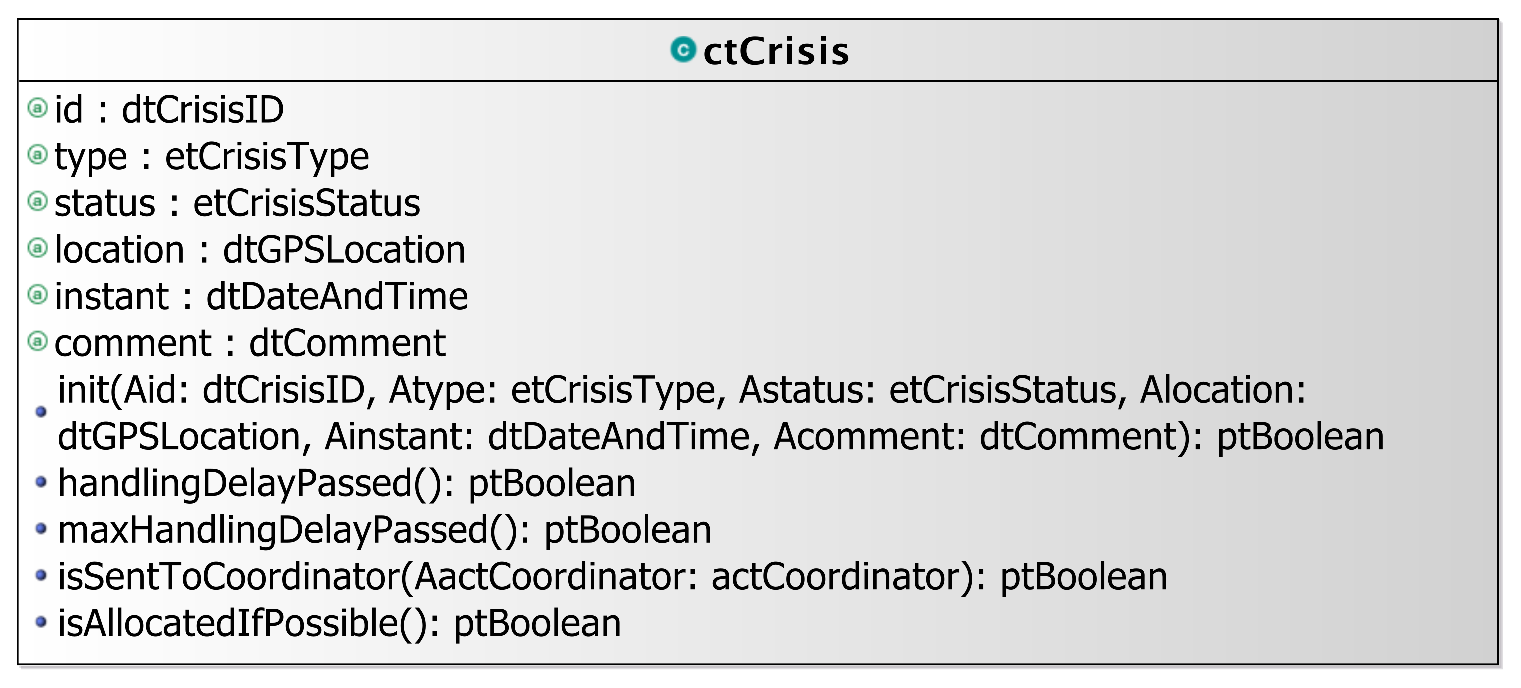
\includegraphics[
angle=0
,scale=0.80
]{./images-report-gen/concept-model/local/PrimaryTypes-Classes/04/cm-pt-ct-lv-04-partc-ctCrisis.eps}
\end{center}
\caption[Concept Model - PrimaryTypes-Classes local view 04 - local view of the ctCrisis primary t]{Concept Model - PrimaryTypes-Classes local view 04. local view of the ctCrisis primary type.}
\label{fig:lu.uni.lassy.excalibur.examples.icrash-CM-view-local-PrimaryTypes-Classes-04}
\end{figure}
\vspace{0.5cm} 


\subsection{Global view 01}
\label{sec:lu.uni.lassy.excalibur.examples.icrash-CM-view-global-PrimaryTypes-Classes-01}
Figure \ref{fig:lu.uni.lassy.excalibur.examples.icrash-CM-view-global-PrimaryTypes-Classes-01} 
shows the global view on primary types class types showing the association(s) types with the actor classes of the environment model.



\begin{figure}[htbp] 
\label{fig:lu.uni.lassy.excalibur.examples.icrash-CM}
\begin{center}
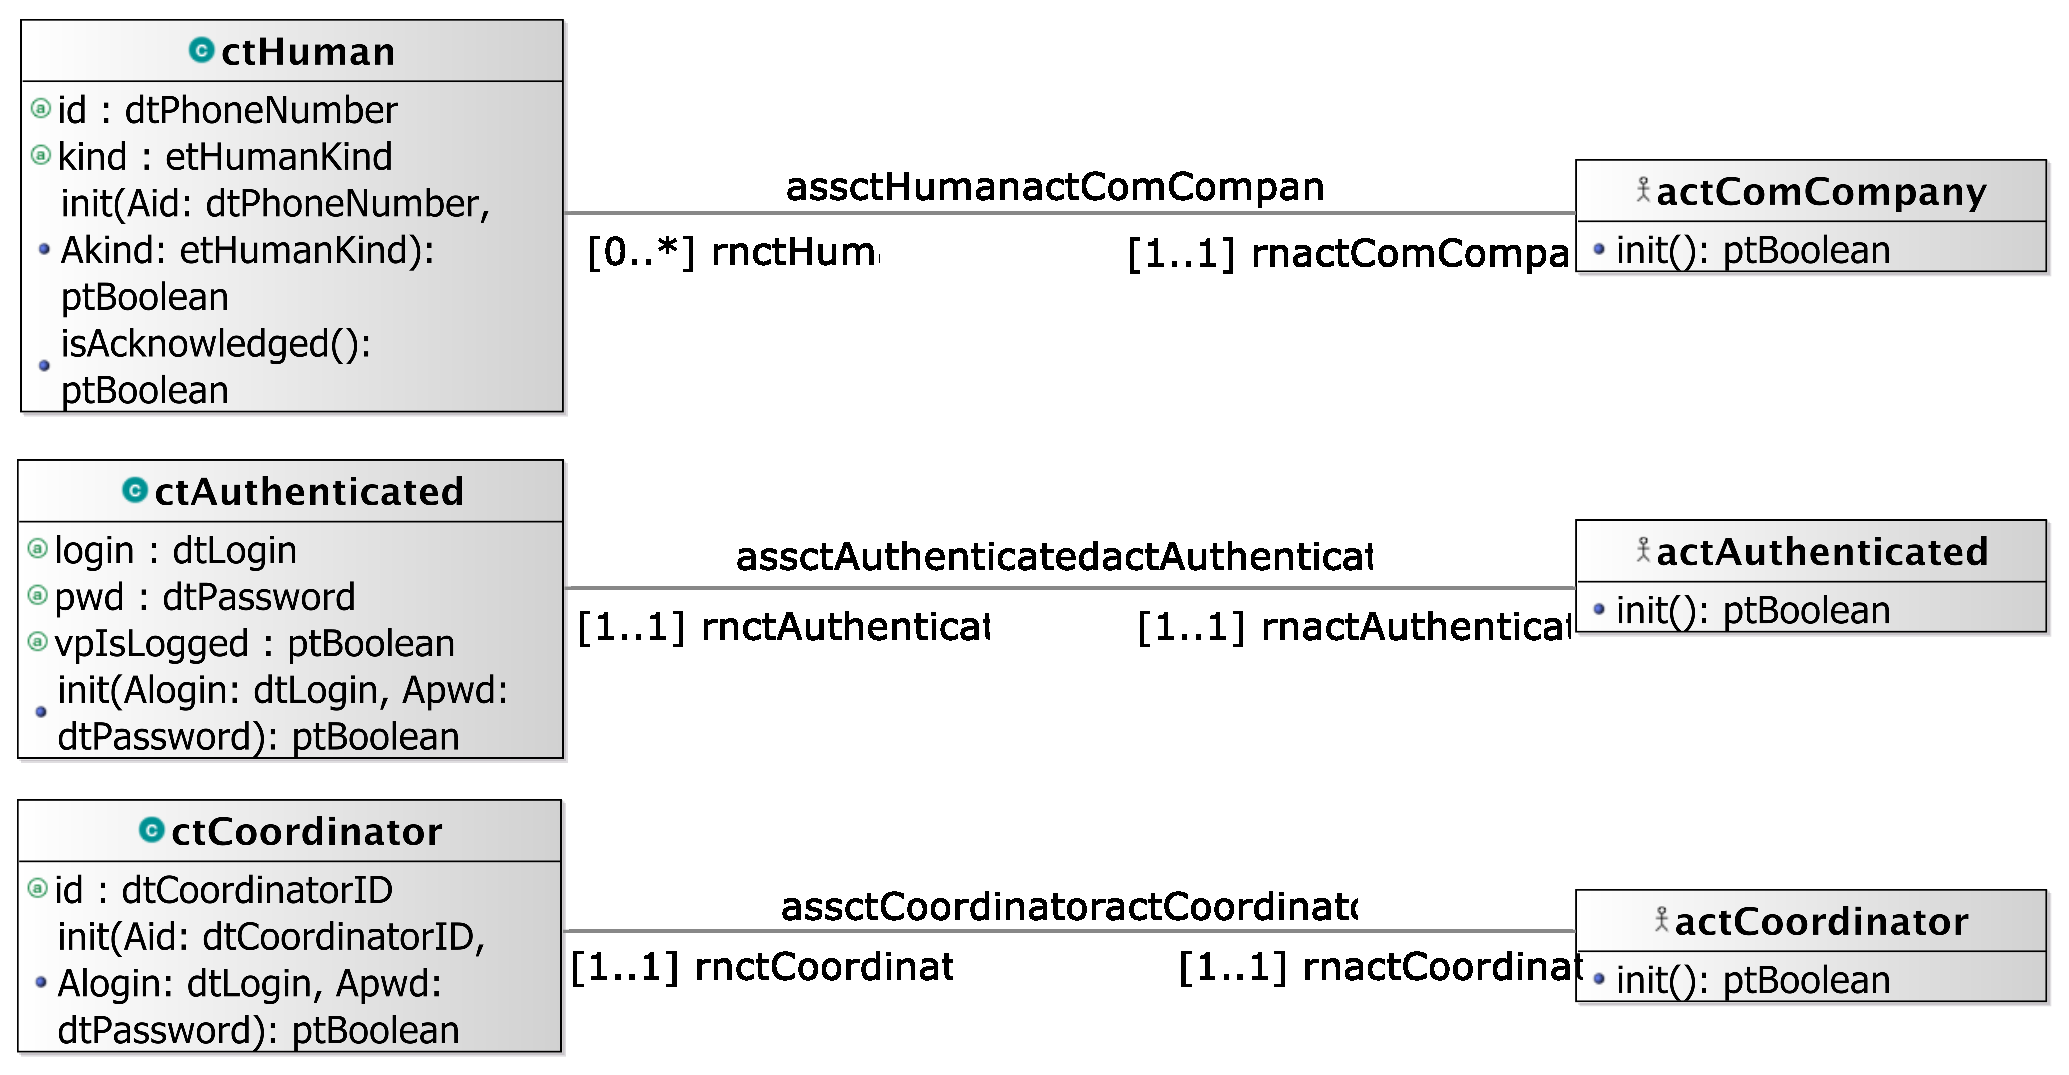
\includegraphics[
angle=0
,width=1.0\textwidth
]{./images-report-gen/concept-model/global/PrimaryTypes-Classes/01/cm-pt-ct-gv-01.eps}
\end{center}
\caption[Concept Model - PrimaryTypes-Classes global view 01 -  Primary types class types global vi]{Concept Model - PrimaryTypes-Classes global view 01.  Primary types class types global view - cm-pt-ct-gv-01
.}
\label{fig:lu.uni.lassy.excalibur.examples.icrash-CM-view-global-PrimaryTypes-Classes-01}
\end{figure}
\vspace{0.5cm} 



\section{PrimaryTypes-Datatypes}
\subsection{Local view 06}
\label{sec:lu.uni.lassy.excalibur.examples.icrash-CM-view-local-PrimaryTypes-Datatypes-06}
Figure \ref{fig:lu.uni.lassy.excalibur.examples.icrash-CM-view-local-PrimaryTypes-Datatypes-06} 



\begin{figure}[htbp] 
\label{fig:lu.uni.lassy.excalibur.examples.icrash-CM}
\begin{center}
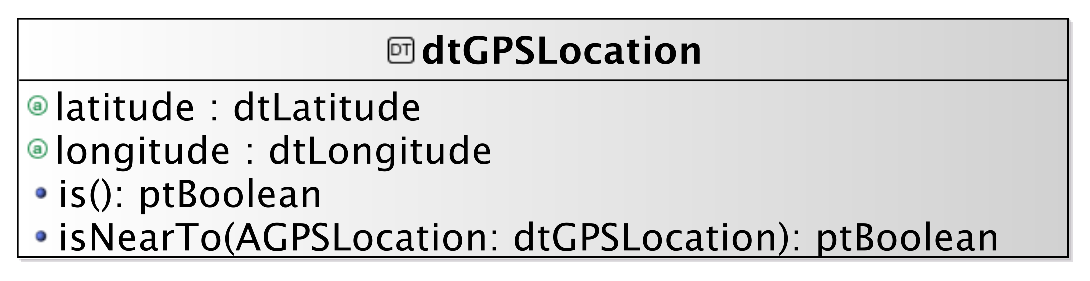
\includegraphics[
angle=0
]{./images-report-gen/concept-model/local/PrimaryTypes-Datatypes/06/cm-pt-dt-lv-02-dtGPSLocation.eps}
\end{center}
\caption[Concept Model - PrimaryTypes-Datatypes local view 06 - ]{Concept Model - PrimaryTypes-Datatypes local view 06. .}
\label{fig:lu.uni.lassy.excalibur.examples.icrash-CM-view-local-PrimaryTypes-Datatypes-06}
\end{figure}
\vspace{0.5cm} 


\subsection{Global view 01}
\label{sec:lu.uni.lassy.excalibur.examples.icrash-CM-view-global-PrimaryTypes-Datatypes-01}
Figure \ref{fig:lu.uni.lassy.excalibur.examples.icrash-CM-view-global-PrimaryTypes-Datatypes-01} 
shows a global view on the \msricrash primary types datatype types.



\begin{figure}[htbp] 
\label{fig:lu.uni.lassy.excalibur.examples.icrash-CM}
\begin{center}
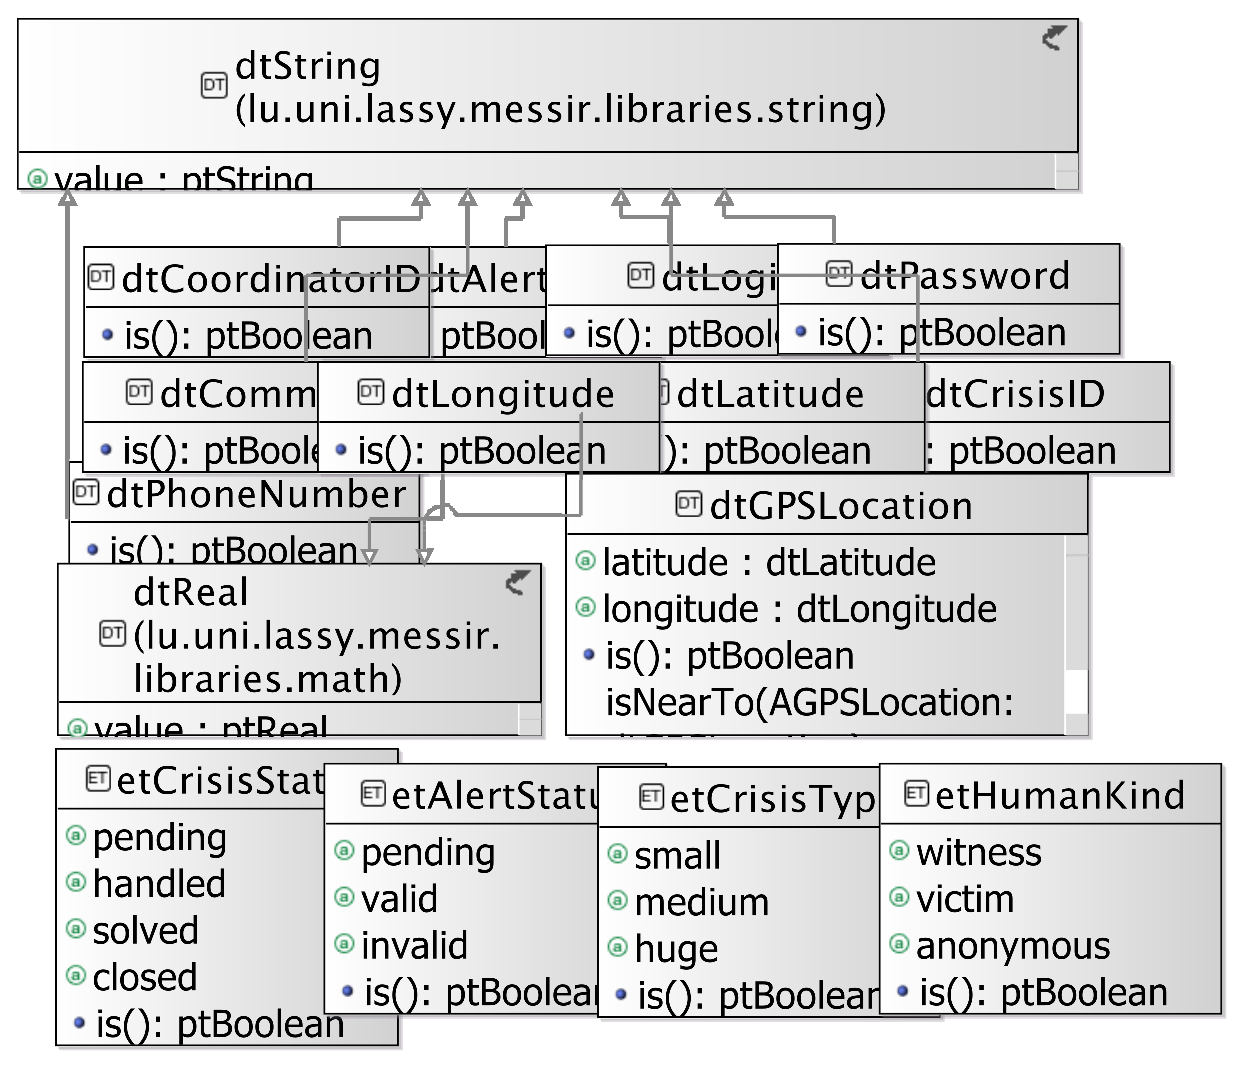
\includegraphics[
angle=0
,width=1.0\textwidth
]{./images-report-gen/concept-model/global/PrimaryTypes-Datatypes/01/cm-pt-dt-gv-01.eps}
\end{center}
\caption[Concept Model - PrimaryTypes-Datatypes global view 01 -  global view of primary types dataty]{Concept Model - PrimaryTypes-Datatypes global view 01.  global view of primary types datatype types - cm-pt-dt-gv-01
.}
\label{fig:lu.uni.lassy.excalibur.examples.icrash-CM-view-global-PrimaryTypes-Datatypes-01}
\end{figure}
\vspace{0.5cm} 





\section{SecondaryTypes-Datatypes}
\subsection{Local view 01}
\label{sec:lu.uni.lassy.excalibur.examples.icrash-CM-view-local-SecondaryTypes-Datatypes-01}
Figure \ref{fig:lu.uni.lassy.excalibur.examples.icrash-CM-view-local-SecondaryTypes-Datatypes-01} shows the local view of the secondary types datatype types.



\begin{figure}[htbp] 
\label{fig:lu.uni.lassy.excalibur.examples.icrash-CM}
\begin{center}
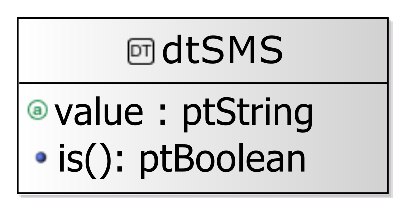
\includegraphics[
angle=0
]{./images-report-gen/concept-model/local/SecondaryTypes-Datatypes/01/cm-st-dt-lv-01.eps}
\end{center}
\caption[Concept Model - SecondaryTypes-Datatypes local view 01 - Local view of the secondary types da]{Concept Model - SecondaryTypes-Datatypes local view 01. Local view of the secondary types datatype types.}
\label{fig:lu.uni.lassy.excalibur.examples.icrash-CM-view-local-SecondaryTypes-Datatypes-01}
\end{figure}
\vspace{0.5cm} 






\section{Concept Model Types Descriptions}
This section provides the textual descriptions of all the types defined in the concept model and that can be part of the graphical views provided.

\subsection{Primary types - Class types descriptions}




The table below is providing comments on the graphical views given for the class types of the primary types. Type logical operations are precisely specified in the operation model.

\begin{datadictionary}
\addheading{Classes}

\adddoublerow{ctAdministrator}{used to caracterize internally the entity that is responsible of administrating the \msricrash system.}
\addsingletwocolumnrow{extends}{icrash.concepts.primarytypes.classes.ctAuthenticated}
\adddoubletwocolumnrow{operation}{\msrcode{init(Alogin:dtLogin, Apwd:dtPassword):ptBoolean}}{used to initialize the current object as a new instance of the ctAdministrator type.}
\adddoublerow{ctAlert}{Used to model crisis alerts sent by any human having communication capability using communication companies belonging to the system's environment}
\adddoubletwocolumnrow{attribute}{\msrcode{comment: dtComment}}{a textual description providing unstructured information on the alert.}
\adddoubletwocolumnrow{attribute}{\msrcode{id: dtAlertID}}{the alert unique identification information.}
\adddoubletwocolumnrow{attribute}{\msrcode{instant: dtDateAndTime}}{the date and time at which the alert notification has been sent.}
\adddoubletwocolumnrow{attribute}{\msrcode{location: dtGPSLocation}}{the position of the alert provided by the space-based satellite navigation system used by the human using the communication company to inform the \msricrash system of a crisis.}
\adddoubletwocolumnrow{attribute}{\msrcode{status: etAlertStatus}}{the alert validation status }
\adddoubletwocolumnrow{operation}{\msrcode{init(Aid:dtAlertID, Astatus:etAlertStatus, Alocation:dtGPSLocation, Ainstant:dtDateAndTime, Acomment:dtComment):ptBoolean}}{used to initialize the current object as a new instance of the ctAlert type.}
\adddoubletwocolumnrow{operation}{\msrcode{isSentToCoordinator(AactCoordinator:actCoordinator):ptBoolean}}{used to provide a given coordinator with current alert information.}
\adddoublerow{ctAuthenticated}{used to model system's representation about actors that need to authenticate to access some specific functionalities.}
\adddoubletwocolumnrow{attribute}{\msrcode{login: dtLogin}}{an identifier for authentication.}
\adddoubletwocolumnrow{attribute}{\msrcode{pwd: dtPassword}}{a key for authentication.}
\adddoubletwocolumnrow{attribute}{\msrcode{vpIsLogged: ptBoolean}}{used to determine the access status.}
\adddoubletwocolumnrow{operation}{\msrcode{init(Alogin:dtLogin, Apwd:dtPassword):ptBoolean}}{used to initialize the current object as a new instance of the ctAuthenticated type.}
\adddoublerow{ctCoordinator}{used to model system's representation about the actors that have the responsibility to handle alerts and crisis.}
\addsingletwocolumnrow{extends}{icrash.concepts.primarytypes.classes.ctAuthenticated}
\adddoubletwocolumnrow{attribute}{\msrcode{id: dtCoordinatorID}}{a unique identification information.}
\adddoubletwocolumnrow{operation}{\msrcode{init(Aid:dtCoordinatorID, Alogin:dtLogin, Apwd:dtPassword):ptBoolean}}{used to initialize the current object as a new instance of the ctCoordinator type.}
\adddoublerow{ctCrisis}{Used to model crisis that are infered from the reception of at least one alert message. Crisis aer entities that are handled by the \msricrash system.}
\adddoubletwocolumnrow{attribute}{\msrcode{comment: dtComment}}{a textual description providing unstructured information on the crisis handling.}
\adddoubletwocolumnrow{attribute}{\msrcode{id: dtCrisisID}}{the crisis unique identification information.}
\adddoubletwocolumnrow{attribute}{\msrcode{instant: dtDateAndTime}}{the date and time at which the first related alert notification has been sent.}
\adddoubletwocolumnrow{attribute}{\msrcode{location: dtGPSLocation}}{the position of the crisis equal by the one of the first alert received and associated to the crisis.}
\adddoubletwocolumnrow{attribute}{\msrcode{status: etCrisisStatus}}{the crisis handling status.}
\adddoubletwocolumnrow{attribute}{\msrcode{type: etCrisisType}}{an indication of the gravity of the crisis.}
\adddoubletwocolumnrow{operation}{\msrcode{handlingDelayPassed():ptBoolean}}{used to determine if the crisis stood too longly in a pending status since last reminder.}
\adddoubletwocolumnrow{operation}{\msrcode{init(Aid:dtCrisisID, Atype:etCrisisType, Astatus:etCrisisStatus, Alocation:dtGPSLocation, Ainstant:dtDateAndTime, Acomment:dtComment):ptBoolean}}{used to initialize the current object as a new instance of the ctAlert type.}
\adddoubletwocolumnrow{operation}{\msrcode{isAllocatedIfPossible():ptBoolean}}{used to allocate a crisis to a coordinator if any or to alert the administrator of crisis waiting to be handled.}
\adddoubletwocolumnrow{operation}{\msrcode{isSentToCoordinator(AactCoordinator:actCoordinator):ptBoolean}}{used to provide a given coordinator with current crisis information.}
\adddoubletwocolumnrow{operation}{\msrcode{maxHandlingDelayPassed():ptBoolean}}{used to determine if the crisis stood too longly in a pending status since its creation.}
\adddoublerow{ctHuman}{used to model system's representation about the indirect actors that has alerted of potential crisis.}
\adddoubletwocolumnrow{attribute}{\msrcode{id: dtPhoneNumber}}{the number of the communication device used to send an alert to \msricrash system.}
\adddoubletwocolumnrow{attribute}{\msrcode{kind: etHumanKind}}{role with respect to the alert notified.}
\adddoubletwocolumnrow{operation}{\msrcode{init(Aid:dtPhoneNumber, Akind:etHumanKind):ptBoolean}}{\msrcode{init}: used to initialize the current object as a new instance of the ctHuman type.}
\adddoublerow{ctState}{used to model the system. Each system specified using \msrmessir must include a ctState class for which there is only one instance at any state of the abstract machine after creation.}
\adddoubletwocolumnrow{attribute}{\msrcode{clock: dtDateAndTime}}{used to represent the system local time.}
\adddoubletwocolumnrow{attribute}{\msrcode{crisisReminderPeriod: dtSecond}}{used to define the delay between two reminders after which a reminder must be sent to the administrator and to the known coordinators to encourage them to handle the crisis.}
\adddoubletwocolumnrow{attribute}{\msrcode{maxCrisisReminderPeriod: dtSecond}}{used to define the maximum delay after which the crisis is ramdomly allocated to a coordinator if any or an alert message is sent to the administrator in order to encourage him to add coordinators.}
\adddoubletwocolumnrow{attribute}{\msrcode{nextValueForAlertID: dtInteger}}{\msrcode{nextValueForAlertID: dtInteger}: used to associate each alert declared with a unique idenitification value. }
\adddoubletwocolumnrow{attribute}{\msrcode{nextValueForCrisisID: dtInteger}}{used to associate each crisis declared with a unique idenitification value. }
\adddoubletwocolumnrow{attribute}{\msrcode{vpLastReminder: dtDateAndTime}}{date and time of the last reminder.}
\adddoubletwocolumnrow{attribute}{\msrcode{vpStarted: ptBoolean}}{used to avoid reacting to an actor message if the system is not started (i.e. oeCreateSystemAndEnvironment not executed).}
\adddoubletwocolumnrow{operation}{\msrcode{init(AnextValueForAlertID:dtInteger, AnextValueForCrisisID:dtInteger, Aclock:dtDateAndTime, AcrisisReminderPeriod:dtSecond, AmaxCrisisReminderPeriod:dtSecond, AvpLastReminder:dtDateAndTime, AvpStarted:ptBoolean):ptBoolean}}{used to initialize the current object as a new instance of the ctState type.}
\end{datadictionary}

\subsection{Primary types - Datatypes types descriptions}



There are no elements in this category in the system analysed.



\subsection{Primary types - Association types descriptions}




The table below is providing comments on the association types of the primary types.

\begin{associationtypes}
\addheading{Undirected associations}
\adddoublerow{assctAlertctCrisis}{a crisis is related to one or more alerts as the alerts judged to concern all the same crisis due to their location. An alert alerts exactly one crisis.}
\adddoublerow{assctAlertctHuman}{ alerts are notified by human through the communication company. We need to keep an internal representation of those human to allow for communication of alert handling.}
\adddoublerow{assctAuthenticatedactAuthenticated}{mainly used to determine if the login request of an authenticated actor can be granted based on the given credentials and the registered ones.}
\adddoublerow{assctCoordinatoractCoordinator}{frequent messages must be sent to coordinator especially in relation to crisis they handle.}
\adddoublerow{assctCrisisctCoordinator}{at any point in time we need to know if a coordinator is handling existing crisis or not.}
\adddoublerow{assctHumanactComCompany}{ in order to communicate with humans who informed about potential crisis, we need to record the communication company to use to send them messages.}
\end{associationtypes}

\subsection{Primary types - Aggregation types descriptions}


There are no aggregation types for the primary types.


\subsubsection{Primary types - Composition types descriptions}



There are no composition types for the primary types.


\input{doc-gen/concept-model/comments-tables/secondaryTypesClasses-comments-table.tex}
\subsection{Secondary types - Datatypes types descriptions}





The table below is providing comments on the graphical views given for the datatype types of the secondary types.

\begin{datadictionary}
\addheading{Datatypes}

\adddoublerow{dtSMS}{a datatype made of a string value used to send textual information to human mobile devices.}
\adddoubletwocolumnrow{attribute}{\msrcode{value: ptString}}{the textual information.}
\adddoubletwocolumnrow{operation}{\msrcode{is():ptBoolean}}{used to determine which strings are considered as valid comments.}
\end{datadictionary}





\subsection{Secondary types - Association types descriptions}



There are no association types for the secondary types.



\subsection{Secondary types - Aggregation types descriptions}



There are no aggregation types for the secondary types.



\subsection{Secondary types - Composition types descriptions}



There are no composition types for the secondary types.





\chapter{Operation Model}
\label{chap:lu.uni.lassy.excalibur.standard.specification.libraries-OM}

This section contains the operation schemes of each operation defined in either an actor, its output interface, in a primary or secondary type (class, datatype or enumeration types). 
The \msrmessir OCL code listing is joined to the comment table.

\lstset{
float,
basicstyle=\scriptsize,
language=Messir,
breakatwhitespace=false,
tabsize=2,
breaklines=true,
numbers=left,
emptylines=1,
numbersep=5pt,
showspaces=false,
showstringspaces=false,
showtabs=false
} 


%% ***************************************************************
%% operations for: Environment-Out Interface Operation Schemes

\section{Environment - Out Interface Operation Schemes}
There are no elements in this category in the system analysed.
		

%% ***************************************************************
%% operations for: Environment-Actor Operation Schemes

\section{Environment - Actor Operation Schemes}
There are no elements in this category in the system analysed.
		

%% ***************************************************************
%% operations for primary type classes

\section{Primary Types - Operation Schemes for Classes}
There are no elements in this category in the system analysed.



%% ***************************************************************
%% operations for primary type datatypes and enumerations

\section{Primary Types - Operation Schemes for Datatypes}
There are no elements in this category in the system analysed.




\section{Primary Types - Operation Schemes for Enumerations}
There are no elements in this category in the system analysed.





%% ***************************************************************
%% operations for secondary type classes


\section{Secondary Types - Operation Schemes for Classes}
There are no elements in this category in the system analysed.




%% ***************************************************************
%% operations for secondary type datatypes and enumerations

\section{Secondary Types - Operation Schemes for Datatypes}
There are no elements in this category in the system analysed.



\section{Secondary Types - Operation Schemes for Enumerations}
There are no elements in this category in the system analysed.





\lstset{
float,
basicstyle=\scriptsize,
language=Messir,
breakatwhitespace=false,
tabsize=2,
breaklines=true,
numbers=left,
emptylines=1,
numbersep=5pt,
showspaces=false,
showstringspaces=false,
showtabs=false
} 

\chapter{Test Model(s)}
\label{chap:lu.uni.lassy.excalibur.standard.specification.libraries-TM}

There are no elements in this category in the system analysed.








\newpage

% Last Modification:
% @author AUTHOR_NAME
% @date TODAY_DATE


\chapter{Additional Constraints}
\label{chap:additional_constraints}
\newpage

%APPENDICES
\appendix
% Last Modification:
% @author AUTHOR_NAME
% @date TODAY_DATE





		
\chapter{Undocumented Messir Specification Elements}











\section[Undocumented Primary Types]{Undocumented Primary Types}


\subsection[Undocumented Primary Datatype Types]{Undocumented Primary Datatype Types}
\begin{itemize}
\item lu.uni.lassy.messir.libraries.calendar.dtDate 
\item lu.uni.lassy.messir.libraries.calendar.dtDateAndTime 
\item lu.uni.lassy.messir.libraries.calendar.dtDay 
\item lu.uni.lassy.messir.libraries.calendar.dtHour 
\item lu.uni.lassy.messir.libraries.math.dtInteger 
\item lu.uni.lassy.messir.libraries.calendar.dtMinute 
\item lu.uni.lassy.messir.libraries.calendar.dtMonth 
\item lu.uni.lassy.messir.libraries.math.dtReal 
\item lu.uni.lassy.messir.libraries.calendar.dtSecond 
\item lu.uni.lassy.messir.libraries.string.dtString 
\item lu.uni.lassy.messir.libraries.calendar.dtTime 
\item lu.uni.lassy.messir.libraries.calendar.dtYear 
\end{itemize}



\subsection[Undocumented Primary Primitive Types]{Undocumented Primary Primitive Types}
\begin{itemize}
\item lu.uni.lassy.messir.libraries.primitives.ptBoolean 
\item lu.uni.lassy.messir.libraries.primitives.ptInteger 
\item lu.uni.lassy.messir.libraries.primitives.ptReal 
\item lu.uni.lassy.messir.libraries.primitives.ptString 
\end{itemize}













\section[Undocumented Operation Specifications]{Undocumented Operation Specifications}
\begin{itemize}
\item lu.uni.lassy.messir.libraries.calendar.dtDate.close 
\item lu.uni.lassy.messir.libraries.calendar.dtDate.eq 
\item lu.uni.lassy.messir.libraries.calendar.dtDate.fromSecondsQty 
\item lu.uni.lassy.messir.libraries.calendar.dtDate.gt 
\item lu.uni.lassy.messir.libraries.calendar.dtDate.is 
\item lu.uni.lassy.messir.libraries.calendar.dtDate.isNow 
\item lu.uni.lassy.messir.libraries.calendar.dtDate.lt 
\item lu.uni.lassy.messir.libraries.calendar.dtDate.toSecondsQty 
\item lu.uni.lassy.messir.libraries.calendar.dtDateAndTime.close 
\item lu.uni.lassy.messir.libraries.calendar.dtDateAndTime.eq 
\item lu.uni.lassy.messir.libraries.calendar.dtDateAndTime.fromSecondsQty 
\item lu.uni.lassy.messir.libraries.calendar.dtDateAndTime.gt 
\item lu.uni.lassy.messir.libraries.calendar.dtDateAndTime.is 
\item lu.uni.lassy.messir.libraries.calendar.dtDateAndTime.isNow 
\item lu.uni.lassy.messir.libraries.calendar.dtDateAndTime.lt 
\item lu.uni.lassy.messir.libraries.calendar.dtDateAndTime.toSecondsQty 
\item lu.uni.lassy.messir.libraries.calendar.dtDay.close 
\item lu.uni.lassy.messir.libraries.calendar.dtDay.is 
\item lu.uni.lassy.messir.libraries.calendar.dtHour.close 
\item lu.uni.lassy.messir.libraries.calendar.dtHour.is 
\item lu.uni.lassy.messir.libraries.math.dtInteger.acos 
\item lu.uni.lassy.messir.libraries.math.dtInteger.add 
\item lu.uni.lassy.messir.libraries.math.dtInteger.asdtReal 
\item lu.uni.lassy.messir.libraries.math.dtInteger.asin 
\item lu.uni.lassy.messir.libraries.math.dtInteger.asptInteger 
\item lu.uni.lassy.messir.libraries.math.dtInteger.atan 
\item lu.uni.lassy.messir.libraries.math.dtInteger.close 
\item lu.uni.lassy.messir.libraries.math.dtInteger.cos 
\item lu.uni.lassy.messir.libraries.math.dtInteger.eq 
\item lu.uni.lassy.messir.libraries.math.dtInteger.frac 
\item lu.uni.lassy.messir.libraries.math.dtInteger.geq 
\item lu.uni.lassy.messir.libraries.math.dtInteger.gt 
\item lu.uni.lassy.messir.libraries.math.dtInteger.is 
\item lu.uni.lassy.messir.libraries.math.dtInteger.leq 
\item lu.uni.lassy.messir.libraries.math.dtInteger.lt 
\item lu.uni.lassy.messir.libraries.math.dtInteger.mod 
\item lu.uni.lassy.messir.libraries.math.dtInteger.msrabs 
\item lu.uni.lassy.messir.libraries.math.dtInteger.msrdiv 
\item lu.uni.lassy.messir.libraries.math.dtInteger.mul 
\item lu.uni.lassy.messir.libraries.math.dtInteger.neq 
\item lu.uni.lassy.messir.libraries.math.dtInteger.opp 
\item lu.uni.lassy.messir.libraries.math.dtInteger.power 
\item lu.uni.lassy.messir.libraries.math.dtInteger.sin 
\item lu.uni.lassy.messir.libraries.math.dtInteger.sqr 
\item lu.uni.lassy.messir.libraries.math.dtInteger.sqrt 
\item lu.uni.lassy.messir.libraries.math.dtInteger.sub 
\item lu.uni.lassy.messir.libraries.math.dtInteger.tan 
\item lu.uni.lassy.messir.libraries.math.dtInteger.toDeg 
\item lu.uni.lassy.messir.libraries.math.dtInteger.toRad 
\item lu.uni.lassy.messir.libraries.math.dtInteger.todtString 
\item lu.uni.lassy.messir.libraries.calendar.dtMinute.close 
\item lu.uni.lassy.messir.libraries.calendar.dtMinute.is 
\item lu.uni.lassy.messir.libraries.calendar.dtMonth.close 
\item lu.uni.lassy.messir.libraries.calendar.dtMonth.is 
\item lu.uni.lassy.messir.libraries.math.dtReal.acos 
\item lu.uni.lassy.messir.libraries.math.dtReal.add 
\item lu.uni.lassy.messir.libraries.math.dtReal.asdtInteger 
\item lu.uni.lassy.messir.libraries.math.dtReal.asin 
\item lu.uni.lassy.messir.libraries.math.dtReal.asptReal 
\item lu.uni.lassy.messir.libraries.math.dtReal.atan 
\item lu.uni.lassy.messir.libraries.math.dtReal.close 
\item lu.uni.lassy.messir.libraries.math.dtReal.cos 
\item lu.uni.lassy.messir.libraries.math.dtReal.eq 
\item lu.uni.lassy.messir.libraries.math.dtReal.frac 
\item lu.uni.lassy.messir.libraries.math.dtReal.geq 
\item lu.uni.lassy.messir.libraries.math.dtReal.gt 
\item lu.uni.lassy.messir.libraries.math.dtReal.is 
\item lu.uni.lassy.messir.libraries.math.dtReal.leq 
\item lu.uni.lassy.messir.libraries.math.dtReal.lt 
\item lu.uni.lassy.messir.libraries.math.dtReal.msrabs 
\item lu.uni.lassy.messir.libraries.math.dtReal.msrdiv 
\item lu.uni.lassy.messir.libraries.math.dtReal.msrround 
\item lu.uni.lassy.messir.libraries.math.dtReal.mul 
\item lu.uni.lassy.messir.libraries.math.dtReal.neq 
\item lu.uni.lassy.messir.libraries.math.dtReal.opp 
\item lu.uni.lassy.messir.libraries.math.dtReal.power 
\item lu.uni.lassy.messir.libraries.math.dtReal.sin 
\item lu.uni.lassy.messir.libraries.math.dtReal.sqr 
\item lu.uni.lassy.messir.libraries.math.dtReal.sqrt 
\item lu.uni.lassy.messir.libraries.math.dtReal.sub 
\item lu.uni.lassy.messir.libraries.math.dtReal.tan 
\item lu.uni.lassy.messir.libraries.math.dtReal.toDeg 
\item lu.uni.lassy.messir.libraries.math.dtReal.toRad 
\item lu.uni.lassy.messir.libraries.math.dtReal.todtString 
\item lu.uni.lassy.messir.libraries.calendar.dtSecond.close 
\item lu.uni.lassy.messir.libraries.calendar.dtSecond.is 
\item lu.uni.lassy.messir.libraries.string.dtString.close 
\item lu.uni.lassy.messir.libraries.string.dtString.dtStringConcat 
\item lu.uni.lassy.messir.libraries.string.dtString.eq 
\item lu.uni.lassy.messir.libraries.string.dtString.geq 
\item lu.uni.lassy.messir.libraries.string.dtString.gt 
\item lu.uni.lassy.messir.libraries.string.dtString.is 
\item lu.uni.lassy.messir.libraries.string.dtString.length 
\item lu.uni.lassy.messir.libraries.string.dtString.leq 
\item lu.uni.lassy.messir.libraries.string.dtString.lt 
\item lu.uni.lassy.messir.libraries.string.dtString.neq 
\item lu.uni.lassy.messir.libraries.string.dtString.subdtString 
\item lu.uni.lassy.messir.libraries.string.dtString.toLower 
\item lu.uni.lassy.messir.libraries.string.dtString.toUpper 
\item lu.uni.lassy.messir.libraries.string.dtString.toptString 
\item lu.uni.lassy.messir.libraries.calendar.dtTime.close 
\item lu.uni.lassy.messir.libraries.calendar.dtTime.eq 
\item lu.uni.lassy.messir.libraries.calendar.dtTime.fromSecondsQty 
\item lu.uni.lassy.messir.libraries.calendar.dtTime.gt 
\item lu.uni.lassy.messir.libraries.calendar.dtTime.is 
\item lu.uni.lassy.messir.libraries.calendar.dtTime.isNow 
\item lu.uni.lassy.messir.libraries.calendar.dtTime.lt 
\item lu.uni.lassy.messir.libraries.calendar.dtTime.toSecondsQty 
\item lu.uni.lassy.messir.libraries.calendar.dtYear.close 
\item lu.uni.lassy.messir.libraries.calendar.dtYear.is 
\item lu.uni.lassy.messir.libraries.primitives.ptBoolean.close 
\item lu.uni.lassy.messir.libraries.primitives.ptBoolean.eq 
\item lu.uni.lassy.messir.libraries.primitives.ptBoolean.is 
\item lu.uni.lassy.messir.libraries.primitives.ptBoolean.msrand 
\item lu.uni.lassy.messir.libraries.primitives.ptBoolean.msrnot 
\item lu.uni.lassy.messir.libraries.primitives.ptBoolean.msror 
\item lu.uni.lassy.messir.libraries.primitives.ptBoolean.msrxor 
\item lu.uni.lassy.messir.libraries.primitives.ptBoolean.neq 
\item lu.uni.lassy.messir.libraries.primitives.ptInteger.acos 
\item lu.uni.lassy.messir.libraries.primitives.ptInteger.add 
\item lu.uni.lassy.messir.libraries.primitives.ptInteger.asin 
\item lu.uni.lassy.messir.libraries.primitives.ptInteger.asptReal 
\item lu.uni.lassy.messir.libraries.primitives.ptInteger.atan 
\item lu.uni.lassy.messir.libraries.primitives.ptInteger.close 
\item lu.uni.lassy.messir.libraries.primitives.ptInteger.cos 
\item lu.uni.lassy.messir.libraries.primitives.ptInteger.eq 
\item lu.uni.lassy.messir.libraries.primitives.ptInteger.frac 
\item lu.uni.lassy.messir.libraries.primitives.ptInteger.geq 
\item lu.uni.lassy.messir.libraries.primitives.ptInteger.gt 
\item lu.uni.lassy.messir.libraries.primitives.ptInteger.is 
\item lu.uni.lassy.messir.libraries.primitives.ptInteger.leq 
\item lu.uni.lassy.messir.libraries.primitives.ptInteger.lt 
\item lu.uni.lassy.messir.libraries.primitives.ptInteger.mod 
\item lu.uni.lassy.messir.libraries.primitives.ptInteger.msrabs 
\item lu.uni.lassy.messir.libraries.primitives.ptInteger.msrdiv 
\item lu.uni.lassy.messir.libraries.primitives.ptInteger.mul 
\item lu.uni.lassy.messir.libraries.primitives.ptInteger.neq 
\item lu.uni.lassy.messir.libraries.primitives.ptInteger.opp 
\item lu.uni.lassy.messir.libraries.primitives.ptInteger.power 
\item lu.uni.lassy.messir.libraries.primitives.ptInteger.sin 
\item lu.uni.lassy.messir.libraries.primitives.ptInteger.sqr 
\item lu.uni.lassy.messir.libraries.primitives.ptInteger.sqrt 
\item lu.uni.lassy.messir.libraries.primitives.ptInteger.sub 
\item lu.uni.lassy.messir.libraries.primitives.ptInteger.tan 
\item lu.uni.lassy.messir.libraries.primitives.ptInteger.toDeg 
\item lu.uni.lassy.messir.libraries.primitives.ptInteger.toRad 
\item lu.uni.lassy.messir.libraries.primitives.ptInteger.toptString 
\item lu.uni.lassy.messir.libraries.primitives.ptReal.acos 
\item lu.uni.lassy.messir.libraries.primitives.ptReal.add 
\item lu.uni.lassy.messir.libraries.primitives.ptReal.asin 
\item lu.uni.lassy.messir.libraries.primitives.ptReal.asptInteger 
\item lu.uni.lassy.messir.libraries.primitives.ptReal.atan 
\item lu.uni.lassy.messir.libraries.primitives.ptReal.close 
\item lu.uni.lassy.messir.libraries.primitives.ptReal.cos 
\item lu.uni.lassy.messir.libraries.primitives.ptReal.eq 
\item lu.uni.lassy.messir.libraries.primitives.ptReal.frac 
\item lu.uni.lassy.messir.libraries.primitives.ptReal.geq 
\item lu.uni.lassy.messir.libraries.primitives.ptReal.gt 
\item lu.uni.lassy.messir.libraries.primitives.ptReal.is 
\item lu.uni.lassy.messir.libraries.primitives.ptReal.leq 
\item lu.uni.lassy.messir.libraries.primitives.ptReal.lt 
\item lu.uni.lassy.messir.libraries.primitives.ptReal.msrabs 
\item lu.uni.lassy.messir.libraries.primitives.ptReal.msrdiv 
\item lu.uni.lassy.messir.libraries.primitives.ptReal.msrround 
\item lu.uni.lassy.messir.libraries.primitives.ptReal.mul 
\item lu.uni.lassy.messir.libraries.primitives.ptReal.neq 
\item lu.uni.lassy.messir.libraries.primitives.ptReal.opp 
\item lu.uni.lassy.messir.libraries.primitives.ptReal.power 
\item lu.uni.lassy.messir.libraries.primitives.ptReal.sin 
\item lu.uni.lassy.messir.libraries.primitives.ptReal.sqr 
\item lu.uni.lassy.messir.libraries.primitives.ptReal.sqrt 
\item lu.uni.lassy.messir.libraries.primitives.ptReal.sub 
\item lu.uni.lassy.messir.libraries.primitives.ptReal.tan 
\item lu.uni.lassy.messir.libraries.primitives.ptReal.toDeg 
\item lu.uni.lassy.messir.libraries.primitives.ptReal.toRad 
\item lu.uni.lassy.messir.libraries.primitives.ptReal.toptString 
\item lu.uni.lassy.messir.libraries.primitives.ptString.close 
\item lu.uni.lassy.messir.libraries.primitives.ptString.eq 
\item lu.uni.lassy.messir.libraries.primitives.ptString.geq 
\item lu.uni.lassy.messir.libraries.primitives.ptString.gt 
\item lu.uni.lassy.messir.libraries.primitives.ptString.is 
\item lu.uni.lassy.messir.libraries.primitives.ptString.length 
\item lu.uni.lassy.messir.libraries.primitives.ptString.leq 
\item lu.uni.lassy.messir.libraries.primitives.ptString.lt 
\item lu.uni.lassy.messir.libraries.primitives.ptString.neq 
\item lu.uni.lassy.messir.libraries.primitives.ptString.ptStringConcat 
\item lu.uni.lassy.messir.libraries.primitives.ptString.subptString 
\item lu.uni.lassy.messir.libraries.primitives.ptString.toLower 
\item lu.uni.lassy.messir.libraries.primitives.ptString.toUpper 
\end{itemize}








 

	\chapter{Specification project lu.uni.lassy.excalibur.examples.icrash}

\label{chap:lu.uni.lassy.excalibur.examples.icrash-lu.uni.lassy.excalibur.examples.icrash}

\section{Use Cases Model}
\label{sec:lu.uni.lassy.excalibur.standard.specification.libraries-gendescr-usecasemodel}

This section contains the use cases elicited during the requirements elicitation phase.
The use cases are textually described as suggested by the \msrmessir method and inspired by the standard Cokburn template~\cite{armour01usecase}.


%% ***************************************************************
%% Use Cases
\subsection{Use Cases}


There are no elements in this category in the system analysed.




%% ***************************************************************
%% Use Case Instances
\pagebreak
\subsection{Use Case Instance(s)}

There are no elements in this category in the system analysed.









	
	\chapter{Messir Specification Files Listing}

\section[File /src-gen/messir-spec/.views.msr]{File ./src-gen/messir-spec/.views.msr}
\scriptsize
\lstinputlisting[style=MessirStyle,firstnumber=auto,captionpos=b,caption={Messir Spec. file .views.msr.}]{./src-gen/messir-spec/.views.msr}
\normalsize
	
\section[File /src-gen/messir-spec/library/calendar.msr]{File ./src-gen/messir-spec/library/calendar.msr}
\scriptsize
\lstinputlisting[style=MessirStyle,firstnumber=auto,captionpos=b,caption={Messir Spec. file calendar.msr.}]{./src-gen/messir-spec/library/calendar.msr}
\normalsize
	
\section[File /src-gen/messir-spec/library/math.msr]{File ./src-gen/messir-spec/library/math.msr}
\scriptsize
\lstinputlisting[style=MessirStyle,firstnumber=auto,captionpos=b,caption={Messir Spec. file math.msr.}]{./src-gen/messir-spec/library/math.msr}
\normalsize
	
\section[File /src-gen/messir-spec/library/primitives.msr]{File ./src-gen/messir-spec/library/primitives.msr}
\scriptsize
\lstinputlisting[style=MessirStyle,firstnumber=auto,captionpos=b,caption={Messir Spec. file primitives.msr.}]{./src-gen/messir-spec/library/primitives.msr}
\normalsize
	
\section[File /src-gen/messir-spec/library/string.msr]{File ./src-gen/messir-spec/library/string.msr}
\scriptsize
\lstinputlisting[style=MessirStyle,firstnumber=auto,captionpos=b,caption={Messir Spec. file string.msr.}]{./src-gen/messir-spec/library/string.msr}
\normalsize
	


	\chapter{Listing of the Prolog Files Referenced in the Operation Model Specification}

\section[File /src-gen/prolog-ref-spec/Operations.../outactActivator-oeSetClock.pl]{File ./src-gen/prolog-ref-spec/Operations/Environment/OUT/outactActivator-oeSetClock.pl}
\scriptsize
\lstinputlisting[style=MessirPrologStyle,firstnumber=auto,captionpos=b,caption={Prolog file outactActivator-oeSetClock.pl.}]{./src-gen/prolog-ref-spec/Operations/Environment/OUT/outactActivator-oeSetClock.pl}
\normalsize
	
\section[File /src-gen/prolog-ref-spec.../outactActivator-oeSollicitateCrisisHandling.pl]{File ./src-gen/prolog-ref-spec/Operations/Environment/OUT/outactActivator-oeSollicitateCrisisHandling.pl}
\scriptsize
\lstinputlisting[style=MessirPrologStyle,firstnumber=auto,captionpos=b,caption={Prolog file outactActivator-oeSollicitateCrisisHandling.pl.}]{./src-gen/prolog-ref-spec/Operations/Environment/OUT/outactActivator-oeSollicitateCrisisHandling.pl}
\normalsize
	
\section[File /src-gen/prolog-ref-spec.../outactAdministrator-oeAddCoordinator.pl]{File ./src-gen/prolog-ref-spec/Operations/Environment/OUT/outactAdministrator-oeAddCoordinator.pl}
\scriptsize
\lstinputlisting[style=MessirPrologStyle,firstnumber=auto,captionpos=b,caption={Prolog file outactAdministrator-oeAddCoordinator.pl.}]{./src-gen/prolog-ref-spec/Operations/Environment/OUT/outactAdministrator-oeAddCoordinator.pl}
\normalsize
	
\section[File /src-gen/prolog-ref-spec.../outactAdministrator-oeDeleteCoordinator.pl]{File ./src-gen/prolog-ref-spec/Operations/Environment/OUT/outactAdministrator-oeDeleteCoordinator.pl}
\scriptsize
\lstinputlisting[style=MessirPrologStyle,firstnumber=auto,captionpos=b,caption={Prolog file outactAdministrator-oeDeleteCoordinator.pl.}]{./src-gen/prolog-ref-spec/Operations/Environment/OUT/outactAdministrator-oeDeleteCoordinator.pl}
\normalsize
	
\section[File /src-gen/prolog-ref-spec/Operations.../outactAuthenticated-oeLogin.pl]{File ./src-gen/prolog-ref-spec/Operations/Environment/OUT/outactAuthenticated-oeLogin.pl}
\scriptsize
\lstinputlisting[style=MessirPrologStyle,firstnumber=auto,captionpos=b,caption={Prolog file outactAuthenticated-oeLogin.pl.}]{./src-gen/prolog-ref-spec/Operations/Environment/OUT/outactAuthenticated-oeLogin.pl}
\normalsize
	
\section[File /src-gen/prolog-ref-spec/Operations.../outactAuthenticated-oeLogout.pl]{File ./src-gen/prolog-ref-spec/Operations/Environment/OUT/outactAuthenticated-oeLogout.pl}
\scriptsize
\lstinputlisting[style=MessirPrologStyle,firstnumber=auto,captionpos=b,caption={Prolog file outactAuthenticated-oeLogout.pl.}]{./src-gen/prolog-ref-spec/Operations/Environment/OUT/outactAuthenticated-oeLogout.pl}
\normalsize
	
\section[File /src-gen/prolog-ref-spec/Operations.../outactComCompany-oeAlert.pl]{File ./src-gen/prolog-ref-spec/Operations/Environment/OUT/outactComCompany-oeAlert.pl}
\scriptsize
\lstinputlisting[style=MessirPrologStyle,firstnumber=auto,captionpos=b,caption={Prolog file outactComCompany-oeAlert.pl.}]{./src-gen/prolog-ref-spec/Operations/Environment/OUT/outactComCompany-oeAlert.pl}
\normalsize
	
\section[File /src-gen/prolog-ref-spec/Operations.../outactCoordinator-oeCloseCrisis.pl]{File ./src-gen/prolog-ref-spec/Operations/Environment/OUT/outactCoordinator-oeCloseCrisis.pl}
\scriptsize
\lstinputlisting[style=MessirPrologStyle,firstnumber=auto,captionpos=b,caption={Prolog file outactCoordinator-oeCloseCrisis.pl.}]{./src-gen/prolog-ref-spec/Operations/Environment/OUT/outactCoordinator-oeCloseCrisis.pl}
\normalsize
	
\section[File /src-gen/prolog-ref-spec/Operations.../outactCoordinator-oeGetAlertsSet.pl]{File ./src-gen/prolog-ref-spec/Operations/Environment/OUT/outactCoordinator-oeGetAlertsSet.pl}
\scriptsize
\lstinputlisting[style=MessirPrologStyle,firstnumber=auto,captionpos=b,caption={Prolog file outactCoordinator-oeGetAlertsSet.pl.}]{./src-gen/prolog-ref-spec/Operations/Environment/OUT/outactCoordinator-oeGetAlertsSet.pl}
\normalsize
	
\section[File /src-gen/prolog-ref-spec/Operations.../outactCoordinator-oeGetCrisisSet.pl]{File ./src-gen/prolog-ref-spec/Operations/Environment/OUT/outactCoordinator-oeGetCrisisSet.pl}
\scriptsize
\lstinputlisting[style=MessirPrologStyle,firstnumber=auto,captionpos=b,caption={Prolog file outactCoordinator-oeGetCrisisSet.pl.}]{./src-gen/prolog-ref-spec/Operations/Environment/OUT/outactCoordinator-oeGetCrisisSet.pl}
\normalsize
	
\section[File /src-gen/prolog-ref-spec.../outactCoordinator-oeInvalidateAlert.pl]{File ./src-gen/prolog-ref-spec/Operations/Environment/OUT/outactCoordinator-oeInvalidateAlert.pl}
\scriptsize
\lstinputlisting[style=MessirPrologStyle,firstnumber=auto,captionpos=b,caption={Prolog file outactCoordinator-oeInvalidateAlert.pl.}]{./src-gen/prolog-ref-spec/Operations/Environment/OUT/outactCoordinator-oeInvalidateAlert.pl}
\normalsize
	
\section[File /src-gen/prolog-ref-spec.../outactCoordinator-oeReportOnCrisis.pl]{File ./src-gen/prolog-ref-spec/Operations/Environment/OUT/outactCoordinator-oeReportOnCrisis.pl}
\scriptsize
\lstinputlisting[style=MessirPrologStyle,firstnumber=auto,captionpos=b,caption={Prolog file outactCoordinator-oeReportOnCrisis.pl.}]{./src-gen/prolog-ref-spec/Operations/Environment/OUT/outactCoordinator-oeReportOnCrisis.pl}
\normalsize
	
\section[File /src-gen/prolog-ref-spec.../outactCoordinator-oeSetCrisisHandler.pl]{File ./src-gen/prolog-ref-spec/Operations/Environment/OUT/outactCoordinator-oeSetCrisisHandler.pl}
\scriptsize
\lstinputlisting[style=MessirPrologStyle,firstnumber=auto,captionpos=b,caption={Prolog file outactCoordinator-oeSetCrisisHandler.pl.}]{./src-gen/prolog-ref-spec/Operations/Environment/OUT/outactCoordinator-oeSetCrisisHandler.pl}
\normalsize
	
\section[File /src-gen/prolog-ref-spec.../outactCoordinator-oeSetCrisisStatus.pl]{File ./src-gen/prolog-ref-spec/Operations/Environment/OUT/outactCoordinator-oeSetCrisisStatus.pl}
\scriptsize
\lstinputlisting[style=MessirPrologStyle,firstnumber=auto,captionpos=b,caption={Prolog file outactCoordinator-oeSetCrisisStatus.pl.}]{./src-gen/prolog-ref-spec/Operations/Environment/OUT/outactCoordinator-oeSetCrisisStatus.pl}
\normalsize
	
\section[File /src-gen/prolog-ref-spec.../outactCoordinator-oeSetCrisisType.pl]{File ./src-gen/prolog-ref-spec/Operations/Environment/OUT/outactCoordinator-oeSetCrisisType.pl}
\scriptsize
\lstinputlisting[style=MessirPrologStyle,firstnumber=auto,captionpos=b,caption={Prolog file outactCoordinator-oeSetCrisisType.pl.}]{./src-gen/prolog-ref-spec/Operations/Environment/OUT/outactCoordinator-oeSetCrisisType.pl}
\normalsize
	
\section[File /src-gen/prolog-ref-spec.../outactCoordinator-oeValidateAlert.pl]{File ./src-gen/prolog-ref-spec/Operations/Environment/OUT/outactCoordinator-oeValidateAlert.pl}
\scriptsize
\lstinputlisting[style=MessirPrologStyle,firstnumber=auto,captionpos=b,caption={Prolog file outactCoordinator-oeValidateAlert.pl.}]{./src-gen/prolog-ref-spec/Operations/Environment/OUT/outactCoordinator-oeValidateAlert.pl}
\normalsize
	
\section[File /src-gen.../outactMsrCreator-oeCreateSystemAndEnvironment.pl]{File ./src-gen/prolog-ref-spec/Operations/Environment/OUT/outactMsrCreator-oeCreateSystemAndEnvironment.pl}
\scriptsize
\lstinputlisting[style=MessirPrologStyle,firstnumber=auto,captionpos=b,caption={Prolog file outactMsrCreator-oeCreateSystemAndEnvironment.pl.}]{./src-gen/prolog-ref-spec/Operations/Environment/OUT/outactMsrCreator-oeCreateSystemAndEnvironment.pl}
\normalsize
	
\section[File /src-gen/prolog-ref-spec.../PrimaryTypesClasses-ctAdministrator-init.pl]{File ./src-gen/prolog-ref-spec/Operations/Concepts/PrimaryTypesClasses/PrimaryTypesClasses-ctAdministrator-init.pl}
\scriptsize
\lstinputlisting[style=MessirPrologStyle,firstnumber=auto,captionpos=b,caption={Prolog file PrimaryTypesClasses-ctAdministrator-init.pl.}]{./src-gen/prolog-ref-spec/Operations/Concepts/PrimaryTypesClasses/PrimaryTypesClasses-ctAdministrator-init.pl}
\normalsize
	
\section[File /src-gen/prolog-ref-spec/Operations.../PrimaryTypesClasses-ctAlert-init.pl]{File ./src-gen/prolog-ref-spec/Operations/Concepts/PrimaryTypesClasses/PrimaryTypesClasses-ctAlert-init.pl}
\scriptsize
\lstinputlisting[style=MessirPrologStyle,firstnumber=auto,captionpos=b,caption={Prolog file PrimaryTypesClasses-ctAlert-init.pl.}]{./src-gen/prolog-ref-spec/Operations/Concepts/PrimaryTypesClasses/PrimaryTypesClasses-ctAlert-init.pl}
\normalsize
	
\section[File /src-gen.../PrimaryTypesClasses-ctAlert-isSentToCoordinator.pl]{File ./src-gen/prolog-ref-spec/Operations/Concepts/PrimaryTypesClasses/PrimaryTypesClasses-ctAlert-isSentToCoordinator.pl}
\scriptsize
\lstinputlisting[style=MessirPrologStyle,firstnumber=auto,captionpos=b,caption={Prolog file PrimaryTypesClasses-ctAlert-isSentToCoordinator.pl.}]{./src-gen/prolog-ref-spec/Operations/Concepts/PrimaryTypesClasses/PrimaryTypesClasses-ctAlert-isSentToCoordinator.pl}
\normalsize
	
\section[File /src-gen/prolog-ref-spec.../PrimaryTypesClasses-ctAuthenticated-init.pl]{File ./src-gen/prolog-ref-spec/Operations/Concepts/PrimaryTypesClasses/PrimaryTypesClasses-ctAuthenticated-init.pl}
\scriptsize
\lstinputlisting[style=MessirPrologStyle,firstnumber=auto,captionpos=b,caption={Prolog file PrimaryTypesClasses-ctAuthenticated-init.pl.}]{./src-gen/prolog-ref-spec/Operations/Concepts/PrimaryTypesClasses/PrimaryTypesClasses-ctAuthenticated-init.pl}
\normalsize
	
\section[File /src-gen/prolog-ref-spec.../PrimaryTypesClasses-ctCoordinator-init.pl]{File ./src-gen/prolog-ref-spec/Operations/Concepts/PrimaryTypesClasses/PrimaryTypesClasses-ctCoordinator-init.pl}
\scriptsize
\lstinputlisting[style=MessirPrologStyle,firstnumber=auto,captionpos=b,caption={Prolog file PrimaryTypesClasses-ctCoordinator-init.pl.}]{./src-gen/prolog-ref-spec/Operations/Concepts/PrimaryTypesClasses/PrimaryTypesClasses-ctCoordinator-init.pl}
\normalsize
	
\section[File /src-gen.../PrimaryTypesClasses-ctCrisis-handlingDelayPassed.pl]{File ./src-gen/prolog-ref-spec/Operations/Concepts/PrimaryTypesClasses/PrimaryTypesClasses-ctCrisis-handlingDelayPassed.pl}
\scriptsize
\lstinputlisting[style=MessirPrologStyle,firstnumber=auto,captionpos=b,caption={Prolog file PrimaryTypesClasses-ctCrisis-handlingDelayPassed.pl.}]{./src-gen/prolog-ref-spec/Operations/Concepts/PrimaryTypesClasses/PrimaryTypesClasses-ctCrisis-handlingDelayPassed.pl}
\normalsize
	
\section[File /src-gen/prolog-ref-spec.../PrimaryTypesClasses-ctCrisis-init.pl]{File ./src-gen/prolog-ref-spec/Operations/Concepts/PrimaryTypesClasses/PrimaryTypesClasses-ctCrisis-init.pl}
\scriptsize
\lstinputlisting[style=MessirPrologStyle,firstnumber=auto,captionpos=b,caption={Prolog file PrimaryTypesClasses-ctCrisis-init.pl.}]{./src-gen/prolog-ref-spec/Operations/Concepts/PrimaryTypesClasses/PrimaryTypesClasses-ctCrisis-init.pl}
\normalsize
	
\section[File /src-gen.../PrimaryTypesClasses-ctCrisis-isAllocatedIfPossible.pl]{File ./src-gen/prolog-ref-spec/Operations/Concepts/PrimaryTypesClasses/PrimaryTypesClasses-ctCrisis-isAllocatedIfPossible.pl}
\scriptsize
\lstinputlisting[style=MessirPrologStyle,firstnumber=auto,captionpos=b,caption={Prolog file PrimaryTypesClasses-ctCrisis-isAllocatedIfPossible.pl.}]{./src-gen/prolog-ref-spec/Operations/Concepts/PrimaryTypesClasses/PrimaryTypesClasses-ctCrisis-isAllocatedIfPossible.pl}
\normalsize
	
\section[File /src-gen.../PrimaryTypesClasses-ctCrisis-isSentToCoordinator.pl]{File ./src-gen/prolog-ref-spec/Operations/Concepts/PrimaryTypesClasses/PrimaryTypesClasses-ctCrisis-isSentToCoordinator.pl}
\scriptsize
\lstinputlisting[style=MessirPrologStyle,firstnumber=auto,captionpos=b,caption={Prolog file PrimaryTypesClasses-ctCrisis-isSentToCoordinator.pl.}]{./src-gen/prolog-ref-spec/Operations/Concepts/PrimaryTypesClasses/PrimaryTypesClasses-ctCrisis-isSentToCoordinator.pl}
\normalsize
	
\section[File /src-gen.../PrimaryTypesClasses-ctCrisis-maxHandlingDelayPassed.pl]{File ./src-gen/prolog-ref-spec/Operations/Concepts/PrimaryTypesClasses/PrimaryTypesClasses-ctCrisis-maxHandlingDelayPassed.pl}
\scriptsize
\lstinputlisting[style=MessirPrologStyle,firstnumber=auto,captionpos=b,caption={Prolog file PrimaryTypesClasses-ctCrisis-maxHandlingDelayPassed.pl.}]{./src-gen/prolog-ref-spec/Operations/Concepts/PrimaryTypesClasses/PrimaryTypesClasses-ctCrisis-maxHandlingDelayPassed.pl}
\normalsize
	
\section[File /src-gen/prolog-ref-spec/Operations.../PrimaryTypesClasses-ctHuman-init.pl]{File ./src-gen/prolog-ref-spec/Operations/Concepts/PrimaryTypesClasses/PrimaryTypesClasses-ctHuman-init.pl}
\scriptsize
\lstinputlisting[style=MessirPrologStyle,firstnumber=auto,captionpos=b,caption={Prolog file PrimaryTypesClasses-ctHuman-init.pl.}]{./src-gen/prolog-ref-spec/Operations/Concepts/PrimaryTypesClasses/PrimaryTypesClasses-ctHuman-init.pl}
\normalsize
	
\section[File /src-gen/prolog-ref-spec.../PrimaryTypesClasses-ctHuman-isAcknowledged.pl]{File ./src-gen/prolog-ref-spec/Operations/Concepts/PrimaryTypesClasses/PrimaryTypesClasses-ctHuman-isAcknowledged.pl}
\scriptsize
\lstinputlisting[style=MessirPrologStyle,firstnumber=auto,captionpos=b,caption={Prolog file PrimaryTypesClasses-ctHuman-isAcknowledged.pl.}]{./src-gen/prolog-ref-spec/Operations/Concepts/PrimaryTypesClasses/PrimaryTypesClasses-ctHuman-isAcknowledged.pl}
\normalsize
	
\section[File /src-gen/prolog-ref-spec/Operations.../PrimaryTypesClasses-ctState-init.pl]{File ./src-gen/prolog-ref-spec/Operations/Concepts/PrimaryTypesClasses/PrimaryTypesClasses-ctState-init.pl}
\scriptsize
\lstinputlisting[style=MessirPrologStyle,firstnumber=auto,captionpos=b,caption={Prolog file PrimaryTypesClasses-ctState-init.pl.}]{./src-gen/prolog-ref-spec/Operations/Concepts/PrimaryTypesClasses/PrimaryTypesClasses-ctState-init.pl}
\normalsize
	
\section[File /src-gen/prolog-ref-spec.../PrimaryTypesDatatypes-dtAlertID-is.pl]{File ./src-gen/prolog-ref-spec/Operations/Concepts/PrimaryTypesDatatypes/PrimaryTypesDatatypes-dtAlertID-is.pl}
\scriptsize
\lstinputlisting[style=MessirPrologStyle,firstnumber=auto,captionpos=b,caption={Prolog file PrimaryTypesDatatypes-dtAlertID-is.pl.}]{./src-gen/prolog-ref-spec/Operations/Concepts/PrimaryTypesDatatypes/PrimaryTypesDatatypes-dtAlertID-is.pl}
\normalsize
	
\section[File /src-gen/prolog-ref-spec.../PrimaryTypesDatatypes-dtComment-is.pl]{File ./src-gen/prolog-ref-spec/Operations/Concepts/PrimaryTypesDatatypes/PrimaryTypesDatatypes-dtComment-is.pl}
\scriptsize
\lstinputlisting[style=MessirPrologStyle,firstnumber=auto,captionpos=b,caption={Prolog file PrimaryTypesDatatypes-dtComment-is.pl.}]{./src-gen/prolog-ref-spec/Operations/Concepts/PrimaryTypesDatatypes/PrimaryTypesDatatypes-dtComment-is.pl}
\normalsize
	
\section[File /src-gen/prolog-ref-spec.../PrimaryTypesDatatypes-dtCoordinatorID-is.pl]{File ./src-gen/prolog-ref-spec/Operations/Concepts/PrimaryTypesDatatypes/PrimaryTypesDatatypes-dtCoordinatorID-is.pl}
\scriptsize
\lstinputlisting[style=MessirPrologStyle,firstnumber=auto,captionpos=b,caption={Prolog file PrimaryTypesDatatypes-dtCoordinatorID-is.pl.}]{./src-gen/prolog-ref-spec/Operations/Concepts/PrimaryTypesDatatypes/PrimaryTypesDatatypes-dtCoordinatorID-is.pl}
\normalsize
	
\section[File /src-gen/prolog-ref-spec.../PrimaryTypesDatatypes-dtCrisisID-is.pl]{File ./src-gen/prolog-ref-spec/Operations/Concepts/PrimaryTypesDatatypes/PrimaryTypesDatatypes-dtCrisisID-is.pl}
\scriptsize
\lstinputlisting[style=MessirPrologStyle,firstnumber=auto,captionpos=b,caption={Prolog file PrimaryTypesDatatypes-dtCrisisID-is.pl.}]{./src-gen/prolog-ref-spec/Operations/Concepts/PrimaryTypesDatatypes/PrimaryTypesDatatypes-dtCrisisID-is.pl}
\normalsize
	
\section[File /src-gen/prolog-ref-spec.../PrimaryTypesDatatypes-dtGPSLocation-is.pl]{File ./src-gen/prolog-ref-spec/Operations/Concepts/PrimaryTypesDatatypes/PrimaryTypesDatatypes-dtGPSLocation-is.pl}
\scriptsize
\lstinputlisting[style=MessirPrologStyle,firstnumber=auto,captionpos=b,caption={Prolog file PrimaryTypesDatatypes-dtGPSLocation-is.pl.}]{./src-gen/prolog-ref-spec/Operations/Concepts/PrimaryTypesDatatypes/PrimaryTypesDatatypes-dtGPSLocation-is.pl}
\normalsize
	
\section[File /src-gen.../PrimaryTypesDatatypes-dtGPSLocation-isNearTo.pl]{File ./src-gen/prolog-ref-spec/Operations/Concepts/PrimaryTypesDatatypes/PrimaryTypesDatatypes-dtGPSLocation-isNearTo.pl}
\scriptsize
\lstinputlisting[style=MessirPrologStyle,firstnumber=auto,captionpos=b,caption={Prolog file PrimaryTypesDatatypes-dtGPSLocation-isNearTo.pl.}]{./src-gen/prolog-ref-spec/Operations/Concepts/PrimaryTypesDatatypes/PrimaryTypesDatatypes-dtGPSLocation-isNearTo.pl}
\normalsize
	
\section[File /src-gen/prolog-ref-spec.../PrimaryTypesDatatypes-dtLatitude-is.pl]{File ./src-gen/prolog-ref-spec/Operations/Concepts/PrimaryTypesDatatypes/PrimaryTypesDatatypes-dtLatitude-is.pl}
\scriptsize
\lstinputlisting[style=MessirPrologStyle,firstnumber=auto,captionpos=b,caption={Prolog file PrimaryTypesDatatypes-dtLatitude-is.pl.}]{./src-gen/prolog-ref-spec/Operations/Concepts/PrimaryTypesDatatypes/PrimaryTypesDatatypes-dtLatitude-is.pl}
\normalsize
	
\section[File /src-gen/prolog-ref-spec/Operations.../PrimaryTypesDatatypes-dtLogin-is.pl]{File ./src-gen/prolog-ref-spec/Operations/Concepts/PrimaryTypesDatatypes/PrimaryTypesDatatypes-dtLogin-is.pl}
\scriptsize
\lstinputlisting[style=MessirPrologStyle,firstnumber=auto,captionpos=b,caption={Prolog file PrimaryTypesDatatypes-dtLogin-is.pl.}]{./src-gen/prolog-ref-spec/Operations/Concepts/PrimaryTypesDatatypes/PrimaryTypesDatatypes-dtLogin-is.pl}
\normalsize
	
\section[File /src-gen/prolog-ref-spec.../PrimaryTypesDatatypes-dtLongitude-is.pl]{File ./src-gen/prolog-ref-spec/Operations/Concepts/PrimaryTypesDatatypes/PrimaryTypesDatatypes-dtLongitude-is.pl}
\scriptsize
\lstinputlisting[style=MessirPrologStyle,firstnumber=auto,captionpos=b,caption={Prolog file PrimaryTypesDatatypes-dtLongitude-is.pl.}]{./src-gen/prolog-ref-spec/Operations/Concepts/PrimaryTypesDatatypes/PrimaryTypesDatatypes-dtLongitude-is.pl}
\normalsize
	
\section[File /src-gen/prolog-ref-spec.../PrimaryTypesDatatypes-dtPassword-is.pl]{File ./src-gen/prolog-ref-spec/Operations/Concepts/PrimaryTypesDatatypes/PrimaryTypesDatatypes-dtPassword-is.pl}
\scriptsize
\lstinputlisting[style=MessirPrologStyle,firstnumber=auto,captionpos=b,caption={Prolog file PrimaryTypesDatatypes-dtPassword-is.pl.}]{./src-gen/prolog-ref-spec/Operations/Concepts/PrimaryTypesDatatypes/PrimaryTypesDatatypes-dtPassword-is.pl}
\normalsize
	
\section[File /src-gen/prolog-ref-spec.../PrimaryTypesDatatypes-dtPhoneNumber-is.pl]{File ./src-gen/prolog-ref-spec/Operations/Concepts/PrimaryTypesDatatypes/PrimaryTypesDatatypes-dtPhoneNumber-is.pl}
\scriptsize
\lstinputlisting[style=MessirPrologStyle,firstnumber=auto,captionpos=b,caption={Prolog file PrimaryTypesDatatypes-dtPhoneNumber-is.pl.}]{./src-gen/prolog-ref-spec/Operations/Concepts/PrimaryTypesDatatypes/PrimaryTypesDatatypes-dtPhoneNumber-is.pl}
\normalsize
	
\section[File /src-gen/prolog-ref-spec.../PrimaryTypesDatatypes-etAlertStatus-is.pl]{File ./src-gen/prolog-ref-spec/Operations/Concepts/PrimaryTypesClasses/PrimaryTypesDatatypes-etAlertStatus-is.pl}
\scriptsize
\lstinputlisting[style=MessirPrologStyle,firstnumber=auto,captionpos=b,caption={Prolog file PrimaryTypesDatatypes-etAlertStatus-is.pl.}]{./src-gen/prolog-ref-spec/Operations/Concepts/PrimaryTypesClasses/PrimaryTypesDatatypes-etAlertStatus-is.pl}
\normalsize
	
\section[File /src-gen/prolog-ref-spec.../PrimaryTypesDatatypes-etCrisisStatus-is.pl]{File ./src-gen/prolog-ref-spec/Operations/Concepts/PrimaryTypesClasses/PrimaryTypesDatatypes-etCrisisStatus-is.pl}
\scriptsize
\lstinputlisting[style=MessirPrologStyle,firstnumber=auto,captionpos=b,caption={Prolog file PrimaryTypesDatatypes-etCrisisStatus-is.pl.}]{./src-gen/prolog-ref-spec/Operations/Concepts/PrimaryTypesClasses/PrimaryTypesDatatypes-etCrisisStatus-is.pl}
\normalsize
	
\section[File /src-gen/prolog-ref-spec.../PrimaryTypesDatatypes-etCrisisType-is.pl]{File ./src-gen/prolog-ref-spec/Operations/Concepts/PrimaryTypesClasses/PrimaryTypesDatatypes-etCrisisType-is.pl}
\scriptsize
\lstinputlisting[style=MessirPrologStyle,firstnumber=auto,captionpos=b,caption={Prolog file PrimaryTypesDatatypes-etCrisisType-is.pl.}]{./src-gen/prolog-ref-spec/Operations/Concepts/PrimaryTypesClasses/PrimaryTypesDatatypes-etCrisisType-is.pl}
\normalsize
	
\section[File /src-gen/prolog-ref-spec.../PrimaryTypesDatatypes-etHumanKind-is.pl]{File ./src-gen/prolog-ref-spec/Operations/Concepts/PrimaryTypesClasses/PrimaryTypesDatatypes-etHumanKind-is.pl}
\scriptsize
\lstinputlisting[style=MessirPrologStyle,firstnumber=auto,captionpos=b,caption={Prolog file PrimaryTypesDatatypes-etHumanKind-is.pl.}]{./src-gen/prolog-ref-spec/Operations/Concepts/PrimaryTypesClasses/PrimaryTypesDatatypes-etHumanKind-is.pl}
\normalsize
	
\section[File /src-gen/prolog-ref-spec/Operations.../SecondaryTypesDatatypes-dtSMS-is.pl]{File ./src-gen/prolog-ref-spec/Operations/Concepts/SecondaryTypesDatatypes/SecondaryTypesDatatypes-dtSMS-is.pl}
\scriptsize
\lstinputlisting[style=MessirPrologStyle,firstnumber=auto,captionpos=b,caption={Prolog file SecondaryTypesDatatypes-dtSMS-is.pl.}]{./src-gen/prolog-ref-spec/Operations/Concepts/SecondaryTypesDatatypes/SecondaryTypesDatatypes-dtSMS-is.pl}
\normalsize
	

	
	

\newpage

%GLOSSARY
\printglossaries
\newpage

%BIBLIOGRAPHY
\cleardoublepage
\bibliographystyle{./../lu.uni.lassy.excalibur.standard.report.libraries/styles/lncs} 
\bibliography{./../lu.uni.lassy.excalibur.standard.report.libraries/defs/references/messir,doc/bibliography/report}
\label{sec:references}

\end{document}
